%! Author = Saeid Yazdani
%! Date = 9/2/2024


\section{\acs{GUI} Operator Software}
\label{sec:gui-operator-software}

The development of a \acs{GUI} application began as a tool to help with
debugging and working on the power supply hardware.
Initially, it was designed to simplify the process of interacting with the
FPGA and managing the various settings and parameters needed to get the
hardware running smoothly.
Over time, the \acs{GUI} was further developed
into a fully functional application that can handle a wide range of tasks
necessary for controlling and managing
the power supply system.
This \acs{GUI} operator software can serve as a reference for the development of
custom operator software, i.e. integrating the \acs{HVS} into
existing \acs{ATE} systems.

\begin{figure}[htbp]
    \centering
    \printfitgraphics[0.62\textheight]{figures/software/gui-main}
    \caption[GUI Operator Main Window]{
        In the main window of the GUI operator, the user quickly input
        settings and values and have a waveform display on top as well as
        multimeter-like reading on the bottom of the window.
    }
    \label{fig:gui-main-window}
\end{figure}

As shown in \autoref{fig:gui-main-window}, one of the primary functions of the
GUI is to allow users to set desired values,
select voltage and current ranges and switch between force voltage and force
current modes, depending on the requirements of the \acs{DUT}.
This makes it easier to adjust the system for different test scenarios
without a need to manually reconfigure everything.

The debug interface within the GUI allows direct reading from and writing to
FPGA registers on byte and bit levels.
This feature is useful for troubleshooting and making precise
adjustments during development and testing as shown in
\autoref{fig:registers-window}.

The register monitor window enables saving and loading of the
FPGA register settings to and from a file
This helps with analysis and diagnosing problems and allows users to reload
these settings back into the FPGA at a later time, if needed.

\begin{figure}[htbp]
    \centering
    \begin{subfigure}[b]{\textwidth}
        \centering
        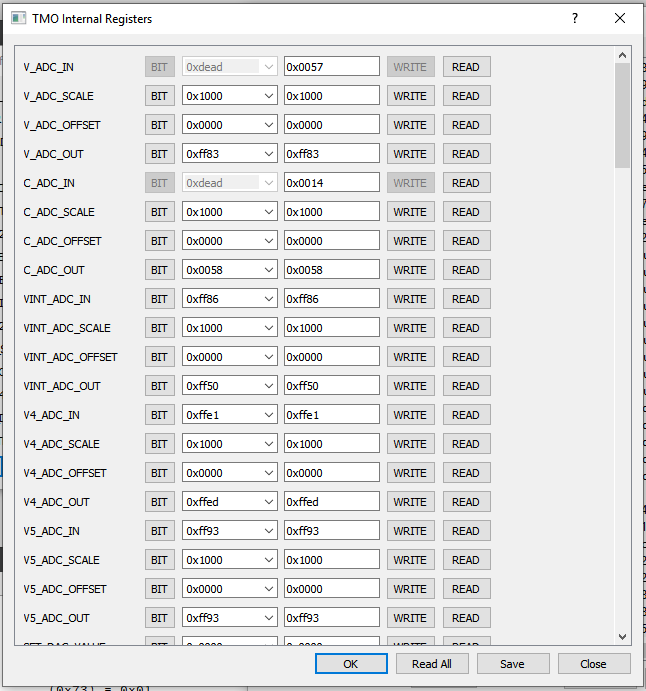
\includegraphics[width=\linewidth,height=0.47\textheight,keepaspectratio]{figures/software/gui-fpga-registers}
        \caption{
            In the registers window, register values are presented to the user on
            an almost realtime basis.
        }
        \label{fig:subfig1}
    \end{subfigure}

    \vspace{0.4em}

    \begin{subfigure}[b]{\textwidth}
        \centering
        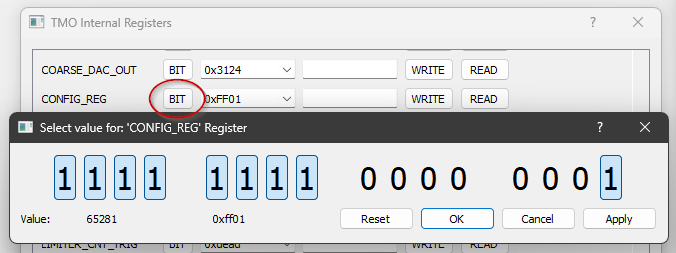
\includegraphics[width=0.86\linewidth,height=0.21\textheight,keepaspectratio]{figures/software/bitselect}
        \caption{
            The bit-level access allows on-the-fly write and read of the
            register bits.
        }
        \label{fig:subfig2}
    \end{subfigure}

    \caption[Register Monitor and Modification Tool]{
        Dedicated register monitor and modify on byte and bit level.
    }
    \label{fig:registers-window}
\end{figure}

Additionally, the GUI serves as an essential interface for loading calibration
data and compensation network (values and timings) data specific to different
loads and DUTs if available. Users can load these data directly from text files
and send it to the FPGA through a serial connection.

An \emph{Event Logging} feature is built into the GUI application that
records all the events and transactions between the user interface
and the system (\autoref{fig:gui-event-logger}).

\begin{figure}[!htbp]
    \centering
    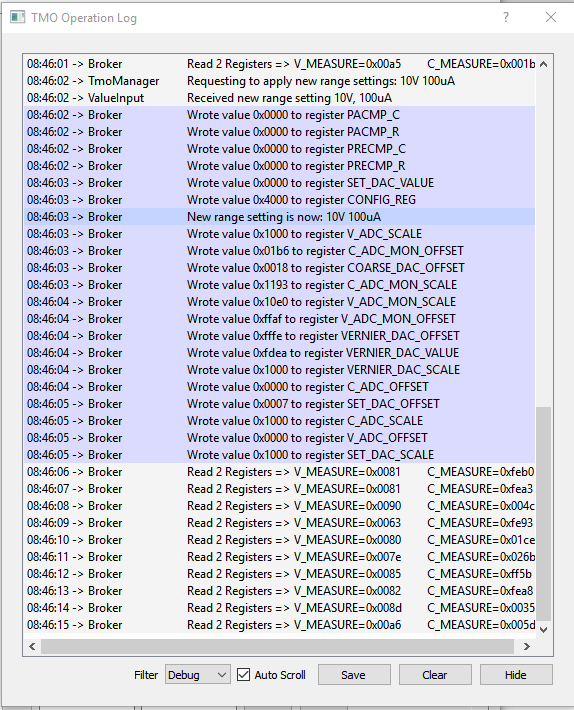
\includegraphics[width=0.62\textwidth]
    {figures/software/gui-logger}
    \caption[GUI Operator Event Logger]{
        The event logger captures all the transactions between the user interface
        and the \acs{HVS} system.
    }
    \label{fig:gui-event-logger}
\end{figure}

The analysis function of the GUI application allows for extracting complete or
partial measurement points from the acquisition memory of the FPGA for
direct analysis on a graph or saving as \acs{CSV} file for offline studies
as shown in \autoref{fig:gui-analysis-form}.

\begin{figure}[!htbp]
    \centering
    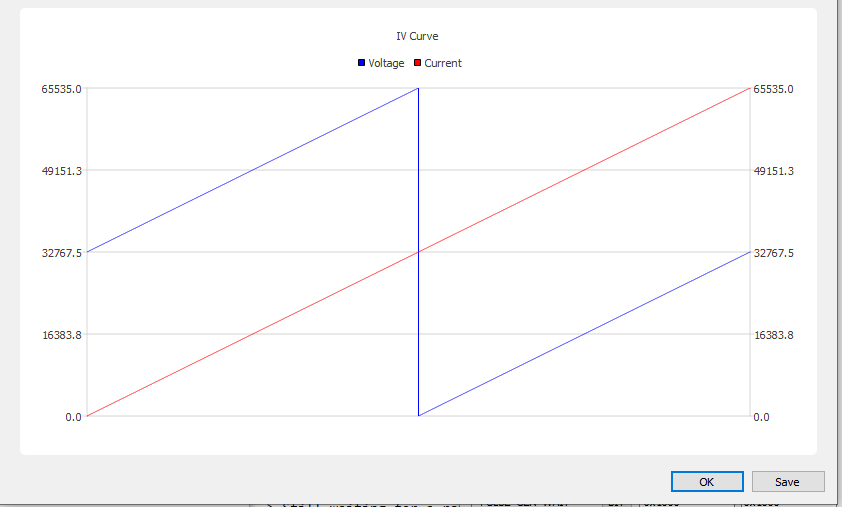
\includegraphics[width=0.72\textwidth]
    {figures/software/gui-stream}
    \caption[GUI Operator Memory Analysis]{
        Partial or full extraction of the acquisition memory in the FPGA
        is provisioned in the operator software.
    }
    \label{fig:gui-analysis-form}
\end{figure}


\begin{figure}[p]
    \centering
    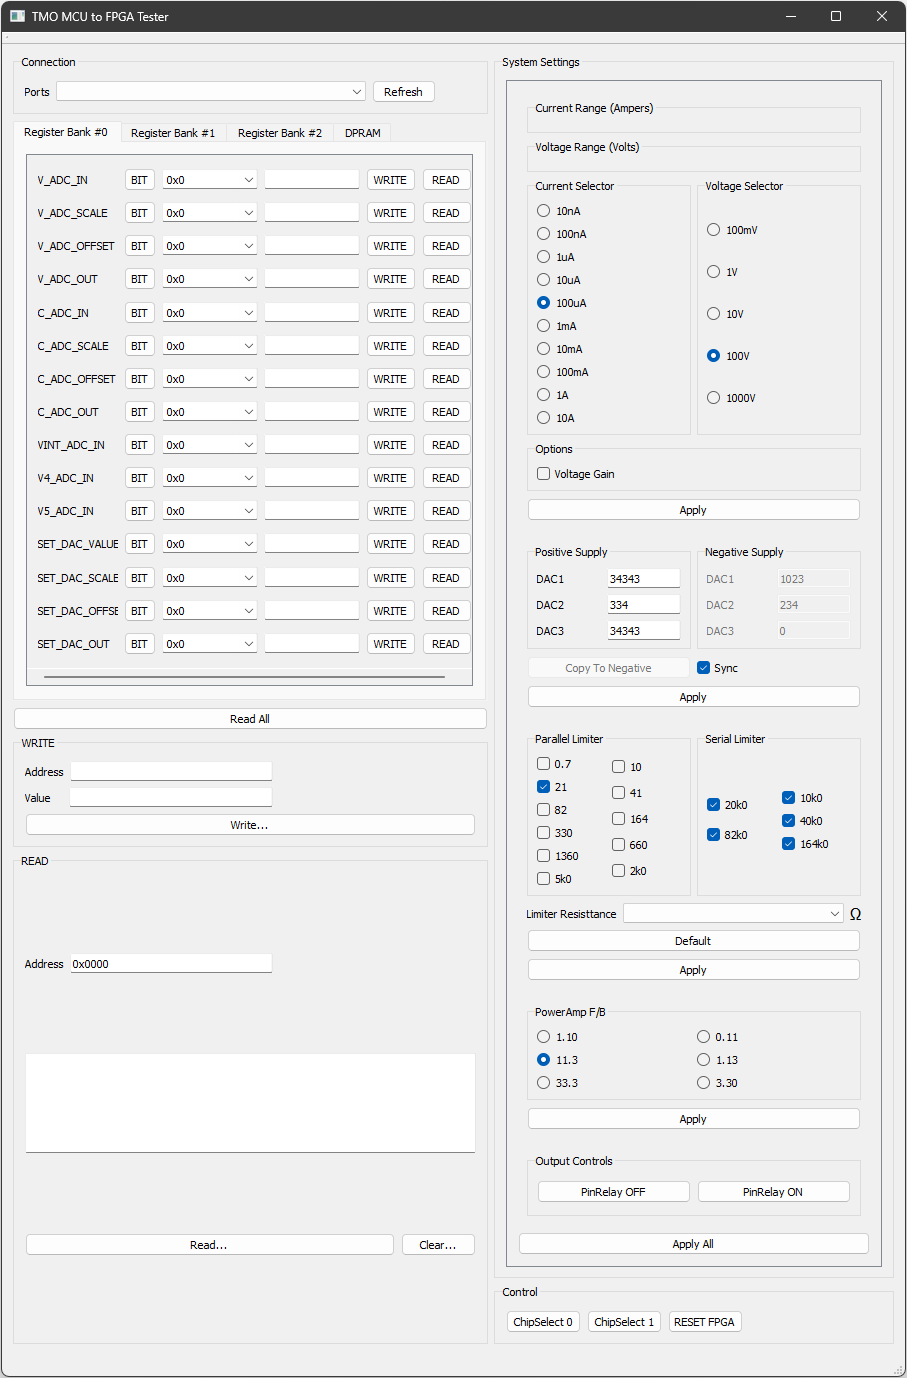
\includegraphics[width=\linewidth,height=0.82\textheight,keepaspectratio]
    {figures/software/debug_window}
    \caption[Direct Control Window]{
        The \emph{Direct Control Window} allows easy control of all modifiable
        hardware and software entities in the system.
    }
    \label{fig:direc-control-window}
\end{figure}
